\section{A New Physical Situation:  Two Masses connected by a Spring}
\label{act2.4.2}
(This activity will get us ready to consider the $PE$ between two atoms or molecules)

\note{}{
You can move this activity along very quickly if you run it as hybrid Small Group/Whole Class activity. Get them up to the board, and read each instruction out loud. Then, don�t give them more than about a minute for each letter prompt. Have someone show/explain the answer, and move right along to the next one. This works pretty well for this activity because most of the questions are short and straightforward. 
Another thing you can do if you are short on time is to have them read and discuss the question for a minute, and then tell you what to put on the board (In effect, you can act as their scribe.)
}
\note{}{The purpose of this activity is to help students make sense of the atom-atom or pair-wise potential introduced in the next activity.  There are three major points that they need to get comfortable with. 
\begin{enumerate} 
\item We are now going to talk about two masses and one spring (no gravity).  We change the coordinate to r, the distance between the masses; and the system oscillates about r0, the equilibrium distance between centers of the masses.  
\item The spring acts like a �normal� spring (PE = 1/2kx2 ) when r has a value close to r0, but becomes different away from r0.  
\item We move the zero of PE to the value of PE when the masses are far apart and where the force is zero.
\end{enumerate}
}
Potential energy curve for two masses connected by a spring:
\note{}{Each group will be making five graphs of PE on their board.  Suggest that they plan ahead so that they have room for all five without having to erase any of them.}

Imagine that we turn off gravity for a moment.  (Or, we go up in the Space Shuttle where things are weightless or very far from all celestial bodies where the force of gravity is very small.)  We have two equal masses (soon we will think of these as atoms or molecules) connected by a spring.

\begin{center}
	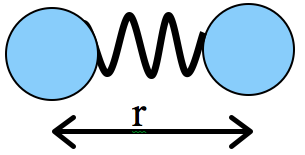
\includegraphics[width=0.25\linewidth]{U2/figs/act242-massandspring}
\end{center}
Both masses move.  The distance $r$ is the separation of the two masses, measured from their centers.  When they are closer together, the spring is compressed and $r$ is smaller; when they are further apart, the spring is stretched and $r$ is larger.  We let the symbol $r_0$ represent the value of $r$ when the spring is neither stretched nor compressed, i.e., the equilibrium position of the masses.
A)	Make a $PE$ graph of the two-mass \& one spring system.
Let's presume for right now that the spring between the masses acts like an ordinary spring that can compress and stretch:
(1)  On the board, sketch a graph of the $PE$ vs.\ $r$ for the two-mass system described above.  Remember what $r_0$ represents and how an ordinary spring behaves when it is stretched or compressed from its equilibrium position.  Since this is an ordinary spring, don't extend the graph into regions of $r$ that are not physically possible.
\note{}{The graph is a parabola centered at r0 and running from zero to infinity (no negative r�s!)}
(2)  Check to make sure that the force as derived from the $PE$ curve is predicted correctly.
(a)	At $r$ = $r_0$, what is the magnitude and direction of the force (i) based on your experience with springs, and (ii) according to the graph of PE? 
(b)	At $r$ > $r_0$, what is the magnitude and direction of the force (i) based on your experience with springs, and (ii) according to the graph of PE? 
(c)	At $r$ \textless  $r_0$, what is the magnitude and direction of the force i) based on your experience with springs, and (ii) according to the graph of $PE$?
\note{}{(2)	The sign of the force is tied to the horizontal axis, i.e., positive forces are in the direction of increasing r (repulsive). Negative forces are in the direction of decreasing r (attractive). They should be fairly comfortable with the idea of attractive and repulsive forces, so the main thing for them to learn here is how to relate those understandings to Force = -slope.}
 
\WCD

B)	Now the spring becomes a little ``weird''
(1)	Imagine that the spring becomes much stronger as the masses get closer - so strong that they can never actually touch.  
Make a new graph on the same axes (don't erase your first graph) of the $PE$ of this new system and be prepared to explain how the shape of the $PE$ curve explains the new weird feature.
\note{}{The graph rises steeply as r approaches the sum of the radii of the two masses.}
(2)	More weirdness:  Now in addition to what you did in (1), assume the spring becomes weaker and weaker as the masses move beyond about $2r_0$.  Then, as $r$ continues to increase, the spring becomes so weak that it has hardly any effect even though the masses are still attached.  The spring is just very, very weak.  
Make a totally new second graph of $PE$ below the first graph that shows both of these new behaviors.  Make sure everyone can use the $PE$ curve to explain both of the new weird features of this two-mass system.
\note{}{Now the slope has to go to zero as r becomes greater than $2r_{0}$.}

\WCD

C)	Making the Graph of the two-mass spring system more useful
Make another  plot of the double weird system on top of the previous graph, but make the spring constant go to zero at a value of the $PE$ that is about twice the previous value.  
Question:  You have just made two graphs with the bottoms of the ``wells'' at the zero of $PE$.  This makes the $PE$ of the two masses for the two springs different when the masses are far apart.  Where could you set the zero of $PE$, so that the $PE$ of both spring systems had the same value when the mass are far apart?  Come to a group consensus and make this combined plot.
\note{}{The �depth of the center parabola part� should be roughly twice as deep as in the previous graphs.  
\\[0.25in]
 The only unique value that all systems will have in common is the value of $PE$ at large separations.  This is one reason this point is chosen.
	Another is that at infinity, it makes sense to say there is no interaction, so $PE = 0$ there seems reasonable, otherwise what number makes sense? ($PE = 37.6$ at $r = \infty$ and no interaction?) 
}

\WCD